\chapter{Formalisation}\label{sec:vp:formalisation}
In this section, we formally define the conceptual structures that comprise the
Virtual Platform. After we have formally defined the structures, we define the
lens functions in terms of this formalisation.

\section{Main Data Structures}
We have a set of features \(\features\), which contain the names of the
features. We also define a set \(\assetcontents\), containing all possible
contents of assets. In our case, the contents are strings, so \(\assetcontents\)
can be seen as the set of all possible strings. Then we have a
set \(\allidentities\) to denote all identities of assets (we will use these identifiers to
identify assets.)

\noindent
We create a notion of \emph{Optional types}, this notation is used to extend a set
with the ``no value'' (\( \bot \)) value:
\[
  \optional{t} = \left\{ \bot \right\} \cup t
\]

\noindent
\( \expressions{\features} \) are expressions over features defined using the
following grammar:
\[
  e \grammarDefinedAs f \mid \hspace*{1mm} \notfeature{e} \mid \truefeature \mid \falsefeature \mid \binopfeature{e}{e}
\]
Here, \( \binopsymbol \in \left\{ \binopand , \binopor , \binopimplies \right\} \)
and \( f \in \features \). The operators are logical conjunctions,
logical disjunctions and logical implications.

\noindent
Asset types are needed to correctly specify different types of assets in the
Virtual Platform:
\[
  \assettype = \left\{ \assetroottype , \assetrepositorytype , \assetfoldertype , \assetfiletype , \assetclasstype , \assetmethodtype , \assetfieldtype , \assetblocktype \right\}
\]

For now, we define feature models or feature trees as a single expression
of type \(\expressions{\features}\). Actual feature models are usually defined
using trees to visualise the hierarchy in them. In the virtual platform, every
asset is allowed to have its own feature model.

\noindent
The set of all assets is denoted using \( \allassets \). Each element 
\(a \in \allassets \) is a tuple of the following type:
\[
  a \in \allidentities \times \assettype \times \powerset{\allassets} \times \optional{\expressions{\features}} \times \expressions{\features} \times \assetcontents
\]

If \( \left( n, t, \mathit{ch}, \mathit{fm}, \mathit{pc}, c \right) \in \allassets \), then \(n\) is the
name, \(t\) is the type of asset, \(\mathit{ch}\) are the children of the asset, 
\(\mathit{fm}\) is the optional feature model, \(\mathit{pc}\) is the presence condition binding
the asset to a feature model and \(c\) is the content of the asset.

Note that the children of assets are defined using a set of assets. The reason
for putting the actual assets in them instead of the identities of the assets
is solely to ease the definitions we will create later.

Another more important point is that we need some way to order the children of
assets. For this, we use a partial ordering on the assets. If we were to not 
have any ordering, the children of an asset could appear in any order. This
means that the contents of those assets (code) will not have a certain order. We do
not want an asset that uses some variable to appear before the asset that 
defines that variable. For this reason, we need an ordering of the set of
assets. 

If we were to put a full ordering on all assets, we would order too much. For
instance, we do not need to compare children of two distinct assets.
Instead, we could introduce a full ordering, but only between the children of
assets. That is, every set of children is ordered. But even this is too strong.
We can restrict the ordering to just children of assets with certain asset
types. The reason for this is that we do not need ordering of children of for
example folder types. It does not matter to us if some file or folder precedes
another file or folder. Following this logic, we only need to place an ordering
on the children of the following asset types: \assetfiletype, \assetclasstype,
\assetmethodtype~ and \assetblocktype. We define the ordering relation on the 
assets as an irreflexive, asymmetric and transitive strict partial order
\(\assetpartialorder\).

To more easily access the properties of assets we define the following
functions:
\[
  \begin{array}{|c|c|}
    \hline
    \namefunc : \unaryFunc{\allassets}{\allidentities} & \typefunc : \unaryFunc{\allassets}{\assettype} \\
    \namefunc \left( \left( n, \_, \_, \_, \_, \_ \right) \right) = n & \typefunc \left( \left( \_, t, \_, \_, \_, \_ \right) \right) = t \\
    \hline 
    \childrenfunc : \unaryFunc{\allassets}{\powerset{\allassets}} & \featuremodelfunc : \unaryFunc{\allassets}{\optional{\expressions{\features}}} \\
    \childrenfunc \left( \left( \_, \_, ch, \_, \_, \_ \right) \right) = ch & \featuremodelfunc \left( \left( \_, \_, \_, fm, \_, \_ \right) \right) = fm \\
    \hline
    \presenceconditionfunc : \unaryFunc{\allassets}{\expressions{\features}} & \contentfunc : \unaryFunc{\allassets}{\assetcontents} \\
    \presenceconditionfunc \left( \left( \_, \_, \_, \_, pc, \_ \right) \right) = pc & \contentfunc \left( \left( \_, \_, \_, \_, \_, c \right) \right) = c \\
    \hline
  \end{array}
\]

A full system in the Virtual Platform is defined as a tuple:
\[
  \virtualplatformtype = \left< \allassets , \features , \allidentities , \assetcontents, \assetpartialorder \right>
\]
This tuple thus contains the assets, the features, the identities and the
contents in the platform, together with a partial order on the assets.

\begin{example}\label{example:basicsystem}
In this example, we will create the running example as described in the background
(Section~\ref{sec:background:example}) in terms of the formalisation described above.
To this end, we need to fill out the tuple that describes a system (\( \virtualplatformtype \)).
This tuple consists of the assets, the features, the identities and the contents.
\end{example}
\begin{figure}
  \centering
  \begin{tikzpicture}
    \treethree{OS}{0}{0}{$f_1$}{$c_1$}{$c_2$}{$c_3$}{}{$\mathit{CLI}$}{$\mathit{logging}$}
  \end{tikzpicture}
  \caption{The example system in the form of an asset tree.}
  \label{fig:example:basicsystem}
\end{figure}
First, we define the set of features, identities and contents. Our codebase
will consist of six assets, so we get six identities and six contents. We only
have two features in our system. For the features, we get \( \features = \left\{ \mathit{logging}, \mathit{CLI} \right\} \),
for the identities, we have \( \allidentities = \left\{ t_1, r_1, f_1, c_1, c_2, c_3 \right\} \)
and finally for the asset contents we have \( \assetcontents = \left\{ s_1, s_2, \dots, s_6 \right\} \).
It can be imagined that these contents are made up off lines of code. Contents
may also be empty in case of for example root, repository, folder of file assets.

Remember that we want the \emph{logging} feature to only be
available when the \emph{CLI} feature is activated, so we create a feature model,
defined by \( \mathit{fm} = \mathit{logging} \binopimplies \mathit{CLI} \).
With this last piece of information we can create the actual assets of the system:
\[
  \begin{array}{ll}
    a_1 = \left( c_1, \assetclasstype, \emptyset, \bot, \truefeature, s_1 \right) & a_4 = \left( f_1, \assetfiletype, \left\{ a_1, a_2, a_3 \right\}, \bot, \truefeature, s_4 \right) \\
    a_2 = \left( c_2, \assetclasstype, \emptyset, \bot, \mathit{CLI}, s_2 \right) & a_5 = \left( r_1, \assetrepositorytype, \left\{ a_4 \right\}, \bot, \truefeature, s_5 \right)\\
    a_3 = \left( c_3, \assetclasstype, \emptyset, \bot, \mathit{logging}, s_3 \right) & a_6 = \left( t_1, \assetroottype, \left\{ a_5 \right\}, \mathit{fm}, \truefeature, s_6 \right)
  \end{array}
\]
We can see that there are only two non-trivial presence conditions, namely in
$a_2$ and $a_3$, which are for the \emph{CLI} and \emph{logging} features,
respectively. We can also see that the feature model (\(\mathit{fm}\)) is
located in the root of the tree ($a_6$). The last part we need to define to
complete the system is the ordering of the assets. There is only one asset
whose children need to be ordered, that is $a_4$. We define the classes to be
ordered such that \(a_1 \assetpartialorder a_2 \assetpartialorder a_3 \).

The asset tree can also be seen in Figure~\ref{fig:example:basicsystem}. This
format is what we will use throughout this work. We have the identities of the
assets as nodes, and the children of these nodes are connected using edges. The edges
are labelled with the presence conditions of the children, but if there is a
non-trivial presence condition.

\section{Parent Functions}\label{sec:vp:parentsfunctions}
Next, we will define a number of functions to find the parent of an asset.
We will need these definitions later to define the restrictions of the platform
and in the definitions of the new operators.
To create this function, we first define a function to retrieve all the parents of an
asset and then define that this function may give back at most one element.
So we first define a function to find the parents of an asset:
\[
  \findparentsfunc : \unaryFunc{\allassets}{\powerset{\allassets}}
\]
\[
  \findparentsfunc \left( a \right) = \left\{ a' \hspace*{1mm} \middle| \hspace*{1mm} a \in \childrenfunc(a') \land a' \in \allassets \right\}
\]

With this definition, we can create the parent function that actually returns
one parent (or none):
\[
  \parentfunc : \unaryFunc{\allassets}{\optional{\allassets}}
\]
\[
  \parentfunc\left( a \right) = 
  \left\{ 
    \begin{array}{ll}
      a' & \text{if } \findparentsfunc(a) = \left\{ a' \right\} \\
      \bot & \text{otherwise}
    \end{array}
  \right.
\]

\section{Restrictions}\label{sec:vp:restrictions}
In this section, we introduce several restrictions to a Virtual Platform
system such that we see it as correct. These restrictions include but are not
limited to, setting up a correct (connected) asset tree.

For a system \( \virtualplatformtype = \left< \allassets , \features , 
\allidentities , \assetcontents \right> \), we first limit how trees are
supposed to be structured. This means that we want any asset to have at most
one parent:
\[
  \forall_{a \in \allassets} \left| \findparentsfunc\left( a \right) \right| \leq 1
\]
Note that we say that the number of parents has to be less than or equal to
one because an asset might have no parent at all (the root asset). We can now
also define that we have only one root asset (the asset tree is connected):
\[
  \left| \left\{ a \hspace*{1mm} \middle| \hspace*{1mm} \left| \findparentsfunc\left( a \right) \right| = 0 \land a \in \allassets \right\} \right| = 1
\]

Finally, we also want to limit the type of assets, some asset types can only
be children of certain other asset types. We start with the root type, which
can only be found at the top of a tree:
\[
  \forall_{a \in \allassets} \typefunc(a) = \assetroottype \Longleftrightarrow \parentfunc(a) = \bot
\]
Note that we do not specify that the root of the tree must be an asset with the
\( \assetroottype \) type. This is because the tree may be cut up by the get
operator that we define later.

The other assets are ordered as follows:
\begin{center}
  \makebox[0cm]{
    \(
      \begin{array}{lcl}
        \forall_{a \in \allassets} \typefunc(a) = \assetroottype & \Longleftrightarrow & \forall_{c \in \childrenfunc(a)} \typefunc(c) = \assetrepositorytype \\
        \forall_{a \in \allassets} \typefunc(a) = \assetrepositorytype & \Longrightarrow & \forall_{c \in \childrenfunc(a)} \typefunc(c) \in \left\{ \assetfoldertype, \assetfiletype \right\} \\
        \forall_{a \in \allassets} \typefunc(a) = \assetfoldertype & \Longrightarrow & \forall_{c \in \childrenfunc(a)} \typefunc(c) \in \left\{ \assetfoldertype, \assetfiletype \right\} \\
        \forall_{a \in \allassets} \typefunc(a) = \assetfiletype & \Longrightarrow & \forall_{c \in \childrenfunc(a)} \typefunc(c) \in \left\{ \assetclasstype, \assetfieldtype, \assetmethodtype, \assetblocktype \right\} \\
        \forall_{a \in \allassets} \typefunc(a) = \assetclasstype & \Longrightarrow & \forall_{c \in \childrenfunc(a)} \typefunc(c) \in \left\{ \assetfieldtype, \assetmethodtype, \assetblocktype \right\} \\
        \forall_{a \in \allassets} \typefunc(a) = \assetmethodtype & \Longrightarrow & \forall_{c \in \childrenfunc(a)} \typefunc(c) = \assetblocktype \\
        \forall_{a \in \allassets} \typefunc(a) = \assetfieldtype & \Longrightarrow & \childrenfunc(a) = \emptyset
      \end{array} 
    \)
  }
\end{center}

\section{Get Operator}\label{sec:vp:getoperator}
We are now ready to define the \emph{get} operator in terms of the
formalisation of the Virtual Platform. Before that let us first look at what
the operator wants to achieve.

The \emph{get} operator wants to create a new asset tree that is a projection
of an input asset tree, the resulting asset tree is created by a \emph{choice}
expression. This choice should be seen as some combination of features that
the user wants to edit. By choosing some combination of features, some code
(read: assets) may not be relevant anymore and thus will not be in the
resulting asset tree. 

We first give the type of the function as follows:
\[
  \vpgetfunc : \binaryFunc{\allassets}{\expressions{\features}}{\optional{\allassets}}
\]
The first argument is the asset on which we want to apply the operator, note
that this does not necessarily have to be the root asset. The second argument
of this function is the so-called \emph{choice}. With this expression, we
``choose'' which features we want to see in the result. Note that the resulting
asset is optional (can be \(\bot\)). This is because the target asset might not
satisfy the given choice, we then result in no asset at all.

The high-level workings of this operator in the Virtual Platform are as
follows. We want to check for each asset if it is relevant for our
\emph{choice}. We do this by checking if the conjunction between an asset its
presence condition and feature model together with the choice is satisfiable.
We can do this satisfiability check using a SAT solver. If this satisfiability
check results as unsatisfiable, the asset is not relevant in our result. We
then do not have to check its children as they are gated by the conditions of
their parents. If it is satisfiable, we include it into our result and 
recursively apply the same strategy to its children. 

Because the asset we apply the operator on might not be the root node of the
tree, we have to be careful of the feature models and presence conditions higher
up in the tree. These conditions might have an impact on the branch our asset is 
on. To account for this, we concatenate all feature models and presence
conditions higher up in the tree. We only have to go through this process for
the asset we apply the operator on, since this impacts all assets further down
in the tree. In the end, the asset we apply the operator on has four parts in
the feature model: the original feature model, the conjunction of all parent
feature models, the conjunction of all the presence ancestral presence
conditions and finally the \emph{choice}.

The recipe described above is for one asset. To make it work for an asset tree,
we apply this function to the children of an asset as well. We only do this
when the satisfiability check was positive. That is, we do not want to check
the children of an asset that we do not want in the first place.

First, we create two functions to ``fold'' all ancestor feature models and
presence conditions. We need these to store them in the target asset its
feature model.
\[
  \foldfmfunc : \unaryFunc{\allassets}{\optional{\expressions{\features}}}
\]
\[
  \foldfmfunc\left(a\right) =
  \left\{
    \begin{array}{ll}
      \featuremodelfunc(a) & \text{if } \parentfunc(a) = \bot \\
      \featuremodelfunc(a) \optional{\land} \foldfmfunc\left( \parentfunc(a) \right) & \text{otherwise}
    \end{array}
  \right.
\]

\[
  \foldpcfunc : \unaryFunc{\allassets}{\expressions{\features}}
\]
\[
  \foldpcfunc\left(a\right) =
  \left\{
    \begin{array}{ll}
      \presenceconditionfunc(a) & \text{if } \parentfunc(a) = \bot \\
      \presenceconditionfunc(a) \land \foldpcfunc\left( \parentfunc(a) \right) & \text{otherwise}
    \end{array}
  \right.
\]
As we can see the above two definitions are quite similar, the only difference
is that presence conditions are not optional where feature models are. So in
the case of feature models we use a ``optional logical conjunction'' 
(\(\optional{\land}\)), which is a simple structure which with we can conjunct
optional expressions:
\[
  e_1 \optional{\land} e_2 =
  \left\{
    \begin{array}{ll}
      e_2 & \text{if } e_1 = \bot \\
      e_1 & \text{if } e_2 = \bot \\
      e_1 \land e_2 & \text{otherwise}
    \end{array}
  \right.
\]

With these definitions, we can create the full definition for the \emph{get}
operator. We create two definitions, the first of which describes the full
operator. The second definition (\(\filterchildrenfunc\)) is used as a helper
function that applies the same general idea but it works on a set of assets.

\[
  \begin{array}{c}
    \vpgetfunc\left( a, e \right) = 
      \left\{
        \begin{array}{ll}
          \left( \namefunc(a), \typefunc(a), \filterchildrenfunc(a, e \land \mathit{fm}'), \mathit{fm}', \presenceconditionfunc(a), \contentfunc(a) \right) & \text{if } e \land \mathit{fm}' \in \sat \\
          \bot & \text{otherwise}
        \end{array}
      \right. \\
      \text{where }\mathit{fm}' = \foldpcfunc\left(a\right) \optional{\land} \foldfmfunc\left(a\right)
  \end{array}
\]

\[
  \begin{array}{c}\def\arraystretch{1.4}
    \filterchildrenfunc : \binaryFunc{\allassets}{\expressions{\features}}{\powerset{\allassets}} \\
    \def\arraystretch{1}
    \filterchildrenfunc(a, e) = 
      \left\{
        (
          n,
          t,
          \filterchildrenfunc(c', \mathit{check}),
          fm,
          pc,
          c
        ) 
        \hspace*{1mm} \middle| \hspace*{1mm}
        \mathit{check} \in \sat 
        \land c' \in \childrenfunc(a) 
      \right\} \\
    \text{where }\mathit{check} = \presenceconditionfunc\left( c' \right) \land e \land \featuremodelfunc\left(c'\right)\text{,} \\
    \text{and }a = \left( n, t, \_, fm, pc, c \right)
  \end{array}
\]

We see that, on the asset that the operator is applied, we change the feature
model to include all of the ancestor presence conditions and feature models.
We do not have to do this in the \(\filterchildrenfunc\) because we know that
the assets we are working with here are not root assets in the resulting asset
tree.

Another observation is that we include the feature model and presence
condition of an asset in the recursive calls. That is, we include the
feature models and the presence conditions in the second argument in calls of
the \(\filterchildrenfunc\). We do this because we know when going into
recursive calls, that these presence conditions and feature models must be
satisfiable, otherwise the current asset would not be in the result.

\begin{example}[Continutation of Example \ref{example:basicsystem}]\label{example:getoperator}
We keep working on the previous example, now we will apply the \emph{get}
operator on the defined asset tree. We look at an application where our choice is the
negation of the \emph{CLI} feature. For simplicity, this \emph{get} operations will
not be called on the root of the tree ($a_6$) but on the file asset ($a_4$).
\end{example}
\begin{figure}
  \centering
  \begin{tikzpicture}
    \treethree{OS}{0}{0}{$f_1$}{$c_1$}{$c_2$}{$c_3$}{}{$\mathit{CLI}$}{$\mathit{logging}$}
    \treeone{OV}{0}{-2.5}{$f'_1$}{$c_1$}{}
    \path[] (OSAS) edge[double,-Stealth] node[left] {$\mathit{get}\left(f_1, \neg\mathit{CLI}\right)$} (OVAN);
  \end{tikzpicture}
  \caption{Example application of the \emph{get} operator with a non-trivial choice.}
  \label{fig:example:get2}
\end{figure}
Again, we call the \emph{get} operator applied to the file asset, with \(\neg\mathit{CLI}\)
as the choice expression: we want to look at the result of \(\vpgetfunc\left(a_4, \neg\mathit{CLI}\right)\).
The result of this application can be seen in Figure~\ref{fig:example:get2}. We see that
the root of the result is now called $f'_1$, this is different because the feature model from
the root is now included in this asset because of the \(\foldfmfunc\), this is the only change
made, as there were no presence conditions to fold with the \(\foldpcfunc\). We also
see that two class assets have been removed from the result. One of these is
obvious, as its presence condition was \emph{CLI}, while we want to have the
negation of it in the result. The other one is because the \emph{logging} feature
requires the \emph{CLI} feature, as stated in the feature model. The checks done are
then are the following: for $a_1$ and $a_4$, we check if \( \mathit{fm} \land \neg\mathit{CLI} \in \sat \),
for $a_2$, we have that \( \mathit{fm} \land \mathit{CLI} \land \neg\mathit{CLI} \not\in \sat \),
hence its absence in the result, this is the same for $a_3$, for which we have that \(\mathit{fm} \land \mathit{logging} \land \neg\mathit{CLI} \not\in \sat\).

\section{Put Operator}\label{sec:vp:putoperator}
In this section, we will introduce the semantics for the put operator for the
Virtual Platform. We first introduce the idea of the operator, then some new 
notation, and then show the formalisation partly in the way we have seen 
before, and partially using pseudocode.

The \emph{put} operator, in a way, does the opposite of the \emph{get} 
operator. We want this operator to include the retrieved asset tree of the
\emph{get} operator back into the original tree on which we applied the
\emph{get} operator. Of course, this tree may have been changed between applying
the two operators, we will even see that if there are no changes, the
\emph{put} operator is trivial.

\subsection*{Distinguishing Assets}
We first create a way to distinguish between the assets in the ``original''
asset tree and the asset tree created after the \emph{get} operator (we will
also refer to this as the ``new'' tree.) This new and old tree have assets in
common, but we know that the \emph{get} operator might have hidden assets, and
the programmer might have added or deleted assets after applying the \emph{get}
operator as well. When we talk about the assets which were there just before
applying the \emph{get} operator, we denote is using \(\oldassets\), knowing
\(\oldassets \subseteq \allassets\). To denote the assets that we want to put
back using the \emph{put} operator, we use \(\newassets\), again with
\(\newassets \subseteq \allassets\). These two sets make up all the assets in
the system: \(\oldassets \cup \newassets = \allassets\).

Uniquely identifying assets should be done using their identifier. However,
when we clone (part of) the asset tree using the \emph{get} operator, the
identifiers do not change. In the \emph{put} operator we can handily use this
to our advantage. With this identifier, we can match ``old'' assets with their
``new'' new counterpart. Thus far we have not put limitations on the identities
of assets, since we did not use them. Now we want to limit the identities such
that they are unique in the old and new asset sets:
\[
  \left| \newassets \right| = \left| \left\{ \namefunc(a) \hspace*{1mm}\middle|\hspace*{1mm} a \in \newassets \right\} \right|
\]
\[
  \left| \oldassets \right| = \left| \left\{ \namefunc(a) \hspace*{1mm}\middle|\hspace*{1mm} a \in \oldassets \right\} \right|
\]
This limitation ensures that any existing asset in the new set will map to
exactly one asset in the old set.

\subsection*{Put By Diff}
Applying the put operator means that we apply the changed assets to the
existing asset tree. One way to do this is by applying a ``diff'' of the tree
much like we have diffs for code in versioning contexts. We identify three
actions that we can apply to assets: we can add, edit and remove them. For each
of these actions we have to make changes to the presence conditions to
correctly apply them when applying the \emph{put} operator:
\begin{itemize}
  \item \textbf{Adding} an asset: Add the ambition to the PC of the new asset.
  \item \textbf{Editing} an asset: Add the ambition to the PC of the new asset,
        and add the negation of the ambition to the old asset.
  \item \textbf{Removing} an asset: Add the negation of the ambition to the old
        asset.
\end{itemize}

At this point, we should realise that there is no difference between the
actions, this is easily visualised in table form, see Table \ref{tab:actions}.
In this table, we can see that the action does not have an effect on what
we do with the presence condition of assets. The only difference is whether we
talk about old or new assets. We do note the ``holes'' in the table, but these
raise no problems. The first hole is when we remove an asset, we have nothing
to do with the new asset. This makes sense as the new asset does not exist
anymore. The way to solve this is by simply ``trying'' to add the ambition to
the presence condition, if this cannot be done, it means that the asset was
removed. Following the same logic, we can simply ``try'' to add the negation
of the ambition to the old asset (we look it up using the unique identifier.)
If this works, we know that the asset was either edited or removed, if this
does not work, the asset was added.
\begin{table}
  \centering
  \begin{tabular}{l|lll} 
              & Added          & Edited            & Removed           \\ \hline
    New asset & PC $\land$ $a$ & PC $\land$ $a$    &                   \\ 
    Old asset &                & PC $\land \neg a$ & PC $\land \neg a$
  \end{tabular}
  \caption{The difference between the result of different actions on assets, $a$ being the ambition}
  \label{tab:actions}
\end{table}
If we can work with this, we only need a set of changed assets for a diff. The
combination of this set and the asset trees makes it possible to correctly
apply the \emph{put} operator. This does mean that we need to record actions
taken on the asset tree after the \emph{get} operator is applied. This is the
least amount of work we can do, however. We need at least some form of diff.
Another option would be to calculate the diff using the old and new asset trees.
This would cost a lot of computing power as we would need to compare every
asset and its contents.

\subsection*{Formalisation}
Now that we have the idea of the \emph{put} laid down, we can create the actual
formalisation.

In Algorithm \ref{alg:vp:put} we can see how the operator works in the form of
an algorithm. We should note the types of the input: first, we have the new 
information, that being the new asset tree (\textit{newAssets}) and the set of
changed assets \textit{changedAssets}, these have the types 
\(\optional{\allassets}\) and \(\powerset{\allidentities}\) respectively. Then
we see the arguments we also had for the \emph{get} operator, being the
original asset tree \textit{oldAssets}, being an element of \(\allassets\) and
the choice expression \textit{choice}, having type \(\expressions{\features}\).
The new expression we have is the \textit{ambition}, having the same type as
the first expression. Finally, as the output of the algorithm, we have the new
asset tree, which we will see, is an altered version of the old asset tree.
The broad idea of the algorithm is as follows. We first find out which assets
we actually need to apply to the old tree, then for each of these assets, we
add the negation of the ambition to the old asset and the ambition to the new
asset. Finally, if there is a new asset (it is not a remove action), we add it
to the old tree. 

To complete these actions we need a number of functions. First up, we need a
function to filter the assets that we actually need to apply, this is the
{\sc FilterAssets} function. To find the old and new assets using its identity,
we have the \(\findoldasset\) and \(\findnewasset\) functions respectively.
Finally, we have the {\sc InsertNewAsset} function to insert the new asset into
the old tree.

The {\sc FilterAssets} function is a function that filters all assets from a
set, which are already children of other assets in that same set. The reason
we want to filter these assets is that we do not need to do anything with
them in the old asset tree. If we have two assets \(a_1\) and \(a_2\), where
\(a_2 \in \childrenfunc(a_1)\) and both of these assets are in the changed
assets, then adding the negation of the ambition to the old version of \(a_1\)
also impacts the old version of \(a_2\) since it is a child of that asset. The
implementation of the function can be found in Algorithm
\ref{alg:vp:filterassets}. The function takes two arguments, one being the
asset we are currently looking at (the identity of it, so its type is
\(\allidentities\).) The other argument is of the same type as the argument we
have seen in the \emph{put} operator: the list of changed assets is a set of
identities (\(\powerset{\allidentities}\)). The function results in a
simplified set of the same type. The function itself works by checking if the
current asset is in the changed assets, if this is the case, all the children
are removed from the changed assets. If it is not the case, the function is
recursively applied to all children of this asset.

The \(\findoldasset\) and \(\findnewasset\) functions are very similar, the goal
of both of these functions is to find the asset with the given identity.
The difference is that, as the names suggest, the \(\findoldasset\) function
looks in the original (old) set of assets (\(\oldassets\)) and the
\(\findnewasset\) function looks in the new set of assets (\(\newassets\)). The
formalisation of these functions is as follows:
\[
  \findassetsfunc_c(i) = \left\{a \hspace*{1mm}\middle|\hspace*{1mm} \namefunc(a) = i \land a \in c \right\}
\]
\[
  \begin{array}{c}
    \findoldasset : \unaryFunc{\allidentities}{\optional{\allassets}} \\ 
    \findoldasset(i) = \left\{
      \begin{array}{ll}
        a & \text{if } \findassetsfunc_{\oldassets}(i) = \left\{ a \right\} \\
        \bot & \text{otherwise}
      \end{array}
    \right.
  \end{array}
\]
\[
  \begin{array}{c}
    \findnewasset : \unaryFunc{\allidentities}{\optional{\allassets}} \\
    \findnewasset(i) = \left\{
      \begin{array}{ll}
        a & \text{if } \findassetsfunc_{\newassets}(i) = \left\{ a \right\} \\
        \bot & \text{otherwise}
      \end{array}
    \right.
  \end{array}
\]

Lastly, we need one more helper function, \(\flattenassetchildren\) does what
its name suggests, it takes an asset and flattens all children within it into a
set. The function is recursively called on the children of the children as
well, such that the result consists of all the assets until the leaves of the
tree.
\[
  \begin{array}{c}
    \flattenassetchildren : \unaryFunc{\allassets}{\powerset{\allassets}} \\
    \flattenassetchildren\left(a\right) = \bigcup \left\{ \left\{ c \right\} \cup \flattenassetchildren\left(c\right) \hspace*{1mm}\middle|\hspace*{1mm} c \in \childrenfunc\left(a\right)\right\}
  \end{array}
\]

\begin{algorithm}
  \caption{{\sc Put}}
  \label{alg:vp:put}
  \begin{algorithmic}[1]
    \item[] {\bf input} \textit{newAssets}: New asset tree (\(\optional{\allassets}\))
    \item[] {\bf input} \textit{changedAssets}: Set of changed assets (\(\powerset{\allidentities}\))
    \item[] {\bf input} \textit{oldAssets}: Original asset tree (\(\allassets\))
    \item[] {\bf input} \textit{choice}: Choice expression (\(\expressions{\features}\))
    \item[] {\bf input} \textit{ambition}: Ambition expression (\(\expressions{\features}\))
    \item[] {\bf output} New asset tree (\(\allassets\))
    \item[]
    \STATE {\it toApply} $\gets$ {\sc FilterAssets}({\it changedAssets}, \namefunc({\it asset}))
    \FORALL {$a \in {\it toApply}$}
      \STATE {\it origAsset} $\gets$ $\findoldasset({\it a})$
      \IF {{\it origAsset} $\neq \bot$}
        \STATE {\it origAsset}.PC $\gets$ {\it origAsset}.PC $\land \neg${\it ambition}
      \ENDIF
      \STATE {\it newAsset} $\gets$ $\findnewasset({\it a})$
      \IF {{\it newAsset} $\neq \bot$}
        \STATE {\it newAsset}.PC $\gets$ {\it newAsset}.PC $\land$ {\it ambition}
        \STATE {\sc InsertNewAsset}({\it newAsset}, {\it origAsset})
      \ENDIF
    \ENDFOR
    \STATE {\bf return} {\it oldAssets}
  \end{algorithmic}
\end{algorithm}

\begin{algorithm}
  \caption{{\sc FilterAssets}}
  \label{alg:vp:filterassets}
  \begin{algorithmic}[1]
    \item[] {\bf input} \textit{changedAssets}: Set of changed assets (\(\powerset{\allidentities}\))
    \item[] {\bf input} \textit{asset}: Root asset (\(\allidentities\))
    \item[] {\bf output} Set of assets (\(\powerset{\allidentities}\))
    \item[]
    \STATE {\it result} $\gets$ {\it changedAssets}
    \IF {{\it asset} $\in$ {\it changedAssets}}
      \STATE {\it newAsset} $\gets \findnewasset\left(asset\right)$
      \IF {{\it newAsset} $= \bot$}
        \STATE {\bf return} {\it result}
      \ENDIF
      \FORALL {{\it c} $\in \flattenassetchildren\left(\mathit{newAsset}\right)$}
        \STATE {\it result} $\gets$ {\it result} $\setminus \namefunc\left(c\right)$
      \ENDFOR
    \ELSE
      \FORALL {{\it c} $\in$ $\childrenfunc(\findnewasset({\it asset})$)}
        \STATE {\it result} $\gets \filterchildrenfunc\left(result, c\right)$
      \ENDFOR
    \ENDIF
    \STATE {\bf return} {\it result}
  \end{algorithmic}
\end{algorithm}

The last function we have yet to define is the {\sc InsertNewAsset} function.
This function is only called when we have either added or edited some asset. In
case of a deletion, we do not have a new asset. Adding an asset can lead to 
problems. For example, in Figure \ref{fig:operator:vp:alignmentproblem}, we start
with an asset tree containing two child assets, of which one
is hidden by applying the \emph{get} operator with $\neg C$ as the
\emph{choice}. The tree is augmented by the programmer by adding a new asset
$a_3$, after $a_1$. Now when the \emph{put} operator is applied on this new
tree, together with the original tree and $B$ as the \emph{ambition}, which leads
to an \emph{Alignment Conflict}. The reason is that we cannot know whether we
want to add the new asset $a_3$ either before or after $a_2$, since $a_2$ was
hidden when we added the new asset. The problem in this case would not be
relevant if the new asset and the hidden asset could not occur simultaneously:
if the final presence condition of the new asset combined with the presence
condition of the hidden asset is not satisfiable, it does not matter whether we
add the new asset before or after the hidden asset. We also do not have to
worry about alignment conflicts when we are working with changes to existing
assets. When we edit an asset, we always want the ``new'' asset to be right
next to the old asset, since that is the exact location where it was before it
was edited. The ``old'' and the ``new'' assets in case of an edit can never
occur at the same time, this is by definition of their presence conditions.

The positioning of children in assets is decided by the partially ordered set
$\assetpartialorder$. In tree forms such as in Figure
\ref{fig:operator:vp:alignmentproblem}, we can visually see the ordering. So we
know that \(a_1 \assetpartialorder a_2\) and later that
\(a_1 \assetpartialorder a_3\). The problem is that these two combined can lead
to two different full orders. We can get \(a_1 \assetpartialorder a_3
\assetpartialorder a_2\), as in the left variant, or \(a_1 \assetpartialorder
a_2 \assetpartialorder a_3\), as seen in the right version. In our algorithm,
the programmer must make sure that this full order ultimately is defined. As
hinted before, this ordering is only relevant for a subset of the asset 
types, we do not want to order assets such as files. 

\begin{figure}
  \centering
  \begin{tikzpicture}
    \node[] (T1R) at (0, 0) {$r_1$};
    \node[] (T1A1) at (-.5,-1) {$a_1$};
    \node[] (T1A2) at (.5,-1) {$a_2$};
    \node[] (T1ANCH) at (0, -1) {};
    \draw[] (T1R) -- (T1A1.north) node [midway, left, yshift=1mm] {$A$};
    \draw[] (T1R) -- (T1A2.north) node [midway, right, yshift=1mm, xshift=-1mm] {$\neg C$};

    \node[] (T2R) at (0,-2.5) {$r_2$};
    \node[] (T2A1) at (0,-3.5) {$a_1$};
    \draw[] (T2R) -- (T2A1.north) node [midway, right] (T2ANCH) {$A$};

    \node[] (T3R) at (5,-2.5) {$r'_2$};
    \node[] (T3A1) at (4.5,-3.5) {$a_1$};
    \node[] (T3A3) at (5.5,-3.5) {$a_3$};
    \node[] (T3ANCH) at (4.2,-3) {};
    \draw[] (T3R) -- (T3A1.north) node [midway, left, yshift=1mm] {$A$};
    \draw[] (T3R) -- (T3A3.north) node [midway, right, yshift=1mm, xshift=-1mm] {};

    \node[] (T4V1R) at (6.5,0) {$r'_1$};
    \node[] (T4V1A1) at (5.5,-1) {$a_1$};
    \node[] (T4V1A2) at (6.5,-1) {$a_2$};
    \node[] (T4V1A3) at (7.5,-1) {$a_3$};
    \draw[] (T4V1R) -- (T4V1A1.north) node [midway, left, yshift=1mm] {$A$};
    \draw[] (T4V1R) -- (T4V1A2.north) node [midway, right, xshift=-1mm] {$\neg C$};
    \draw[] (T4V1R) -- (T4V1A3.north) node [midway, right, yshift=1mm] {$B$};

    \node[] (T4V2R) at (3.5,0) {$r'_1$};
    \node[] (T4V2A1) at (2.5,-1) {$a_1$};
    \node[] (T4V2A3) at (3.5,-1) {$a_3$};
    \node[] (T4V2A2) at (4.5,-1) {$a_2$};
    \draw[] (T4V2R) -- (T4V2A1.north) node [midway, left, yshift=1mm] {$A$};
    \draw[] (T4V2R) -- (T4V2A3.north) node [midway, right, xshift=-1mm] {$B$};
    \draw[] (T4V2R) -- (T4V2A2.north) node [midway, right, yshift=1mm] {$\neg C$};

    \node[coordinate] (T3T4MANCH) at (5,-1.75) {};

    \draw[double,-Stealth] (T1ANCH) -- (T2R) node [midway, left] {$\textit{get}\left(r_1, C\right)$};
    \draw[double,-Stealth] (T2ANCH) -- (T3ANCH) node [midway, below] {Add $a_3$};
    \path[] (T3R.north) edge[double] node [midway, right] {} (T3T4MANCH);
    \path[] (T3T4MANCH.north) edge[double,-Stealth,bend right=-10] node[right, yshift=-5mm, xshift=-5mm] {$\textit{put}\left(r'_2, \left\{ a_3 \right\}, r_1, C, B\right)$} (T4V1A2); 
    \path[] (T3T4MANCH.north) edge[double,-Stealth,bend left=-10] node[] {} (T4V2A3); 
  \end{tikzpicture}
  \caption{Example of how an alignment conflict might arise.}
  \label{fig:operator:vp:alignmentproblem}
\end{figure}

In the end, we want our function to first check the type of the parent asset.
If the ordering of that parent is not relevant, we can simply add the asset to
the ``new'' tree without a problem. Otherwise, we need to check if the action
performed on the given asset is an edit of an asset or an addition of a 
completely new asset. In the case of an edit, we can automatically restore the
ordering of the children (we simply add the new asset right next to the
``old'' variant.) In the other case, the programmer manually needs to restore
the ordering of the children. This procedure is shown in the form of an
algorithm in Algorithm \ref{alg:vp:insertnewasset}. 

\begin{algorithm}
  \caption{{\sc InsertNewAsset}}
  \label{alg:vp:insertnewasset}
  \begin{algorithmic}[1]
    \item[] {\bf input} \textit{newAsset}: The asset to insert (\(\allassets\))
    \item[] {\bf input} \textit{oldAsset}: Optional ``old'' asset (\(\optional{\allassets}\))
    \item[]
    \STATE $\textit{newParent} \gets \findoldasset(\parentfunc(\textit{newAsset}))$ \label{alg:insertnewasset:insertion1}
    \STATE $\childrenfunc(\textit{newParent}) \gets \childrenfunc(\textit{newParent}) \cup \left\{ \textit{newAsset} \right\}$ \label{alg:insertnewasset:insertion2}
    \IF {\typefunc(\parentfunc({\it newAsset})) $\in \left\{ \assetclasstype, \assetmethodtype, \assetblocktype, \assetfiletype \right\}$ }
      \IF {$\textit{oldAsset} = \bot$}
        \STATE {\bf Manually repair full ordering of children of} {\it newParent} \label{alg:insertnewasset:manualrepair}
      \ELSE
        \FORALL {$a \in \childrenfunc(\textit{newParent})$} \label{alg:insertnewasset:startordering}
          \IF {$\textit{oldAsset} \assetpartialorder a$}
            \STATE {\bf define} $\textit{newAsset} \assetpartialorder a$
          \ENDIF
        \ENDFOR \label{alg:insertnewasset:endordering}
      \ENDIF  
    \ENDIF
  \end{algorithmic}
\end{algorithm}

In the algorithm we first see the new asset getting added to the ``old'' asset
tree (lines \ref{alg:insertnewasset:insertion1} and
\ref{alg:insertnewasset:insertion2}). In case the ordering is irrelevant, the
function ends here. Otherwise, we need to manually repair the full ordering in
case of a completely new asset (line \ref{alg:insertnewasset:manualrepair}), or
we programmatically set the new ordering in case of an edit action (lines
\ref{alg:insertnewasset:startordering} until
\ref{alg:insertnewasset:endordering}).

A final remark on the process of the \emph{put} operator is that we do not do
anything with the folded feature models and presence conditions that were put
in the feature model of the resulting root asset of the \emph{get} operator.
We do not process this change after applying the \emph{put} operator because
these changes are not fundamentally incorrect, even when they are copied over
to the original tree. Note that this copying over can only happen when the root
of the new tree is changed, which will most definitely be an uncommon occurrence.
The copying over is not fundamentally wrong since, at this point of the asset
tree, we already know that the conditions in this feature model must hold (they
came from ancestors.) It is valid to simplify a feature model at some point in
an asset tree if (part of) it can already be concluded from feature models and
presence conditions higher up in the tree. If this simplification is always
attempted at all assets in the tree, the ``not cleaning up'' of the feature
models is irrelevant.

\begin{figure}
  \centering
  \begin{tikzpicture}
    \treethree{OS}{0}{0}{$f_1$}{$c_1$}{$c_2$}{$c_3$}{}{$\mathit{C}$}{$\mathit{L}$}
    \treeone{OV}{0}{-3.5}{$f_2$}{$c_1$}{}
    \treetwo{EV}{4}{-3.5}{$f'_2$}{$c_1$}{$c_4$}{}{}
    \node[] (M1) at (4.5, -5.2) {$m_1$};
    \path[] (EVA2.south) edge[] (M1.north);

    \node[] (ESR) at (4, 0) {$f'_1$};
    \node[] (ESA1) at (2.4, -1) {$c_1$};
    \node[] (ESA2) at (3.2, -1) {$c'_1$};
    \node[] (ESA3) at (4, -1) {$c_4$};
    \node[] (ESA4) at (4.8, -1) {$c_2$};
    \node[] (ESA5) at (5.6, -1) {$c_3$};
    \node[] (ESA6) at (4, -1.7) {$m_1$};
    \draw[] (ESA3) -- (ESA6.north);
    \draw[] (ESR) -- (ESA1.north) node [midway, left, yshift=1mm] {$\neg\mathit{G}$};
    \draw[] (ESR) -- (ESA2.north) node [midway, right] {$\mathit{G}$};
    \draw[] (ESR) -- (ESA3.north) node [midway, right] {$\mathit{G}$};
    \draw[] (ESR) -- (ESA4.north) node [midway, right] {$\mathit{C}$};
    \draw[] (ESR) -- (ESA5.north) node [midway, right, yshift=1mm] {$\mathit{L}$};

    \path[] (OSAS) edge[double,-Stealth] node[left] {$\mathit{get}\left(f_1, \neg\mathit{C}\right)$} (OVAN);
    \path[] (EVAN) edge[double,-Stealth] node[right] {$\mathit{put}\left(f'_2, \left\{ c_1, c_4, m_1 \right\}, f_1, \neg\mathit{C}, \mathit{G}\right)$} (4, -2);
    \path[] (OVAE) edge[double,-Stealth] node[below] {Actual Edit} (EVAW);
  \end{tikzpicture}
  \caption{Example application of the \emph{put} operator.}
  \label{fig:example:put}
\end{figure}

\begin{example}[Continuation of Example \ref{example:getoperator}]
  We continue the example in which we applied the \emph{get} operator to the
  system we introduced even before that. Specifically, we will continue the
  second example where we applied the \emph{get} operator with as choice
  expression \(\neg\mathit{CLI}\). An overview can be seen in Figure~\ref{fig:example:put}.
  Note that we shortened the names of the features to their first letters.
The actual edit this time is to add a new feature called \emph{GUI} (in the
figure shortened to just \emph{G}.) For this, we have to edit $a_1$ (identified
by $c_1$) and we have to add two new assets identified by $c_4$ and $m_1$,
respectively. The latter addition is a child of the first one. Now when we apply
the \emph{put} operator, we apply it with as ambition \emph{G}, since we want
these changes to apply to the \emph{GUI} feature. The operator first filters the
changed assets set to only contain the relevant assets. This filter removes $m_1$
from the set since it is a child of $c_4$, it will be automatically applied when
applying $c_4$. We first apply $c_1$, which is simple as it is just an edit action.
The old asset from the original tree used to have the trivial presence condition,
this becomes the negation of the ambition. The new version of $c_1$, in the result
identified as $c'_1$, gets as presence condition the ambition. Lastly, we need to
apply $c_4$, this leads to an alignment conflict as we do not know if we should add
it before $c_2$, after $c_2$ or after $c_3$. We decide to put it right after $c'_1$.
This new asset also gets the ambition as its presence condition.
\end{example}